\chapter{Related Work}
\label{ch:relatedwork}

\section{Disk-based Graph ANN}

Approximate nearest neighbor search for high-dimensional vectors has been studied through tree-based\cite{muja2014flann}, hashing-based\cite{datar2004lsh}, clustering-based\cite{chen2021spann}, and graph-based indexes\cite{malkov2020hnsw,fu2019nsg}.
Graph-based methods are widely used because they provide strong empirical tradeoffs between recall and search efficiency.
Product quantization (PQ)\cite{jegou2011pq} and optimized product quantization (OPQ)\cite{ge2013opq} are often combined with these indexes to reduce memory and computation cost.
However, fully in-memory graph indexes still require substantial memory for raw vectors and graph structure, making them difficult to scale to hundreds of millions of points\cite{subramanya2019diskann}.

DiskANN addresses this problem by keeping PQ-compressed navigation vectors in memory while storing full graph records on SSD\cite{subramanya2019diskann}.
It has been adopted in practical vector databases and cloud services\cite{wang2021milvus,upreti2025cosmos}.
DiskANN++ further improves disk-based graph search with query-sensitive entry points and page-based traversal\cite{ni2023diskannpp}.
Despite these advances, DiskANN-style systems still issue many random SSD reads during beam search.
PipeANN reduces the latency of a single query by overlapping computation and SSD I/O through pipelining\cite{osdi25pipeann}.
PaceANN targets the same disk bottleneck from a different angle: instead of hiding I/O latency, it reduces redundant I/O under high concurrency through adaptive caching and early termination.

Figure~\ref{fig:diskann-layout} summarizes why node expansion is expensive in DiskANN.
Each node is stored as a fixed-length disk record containing its full-precision vector and neighbor list, so expanding a node usually requires a 4\,KB random read.
PaceANN's mechanisms directly reduce how often this path is taken.

\begin{figure}[htbp]
  \centering
  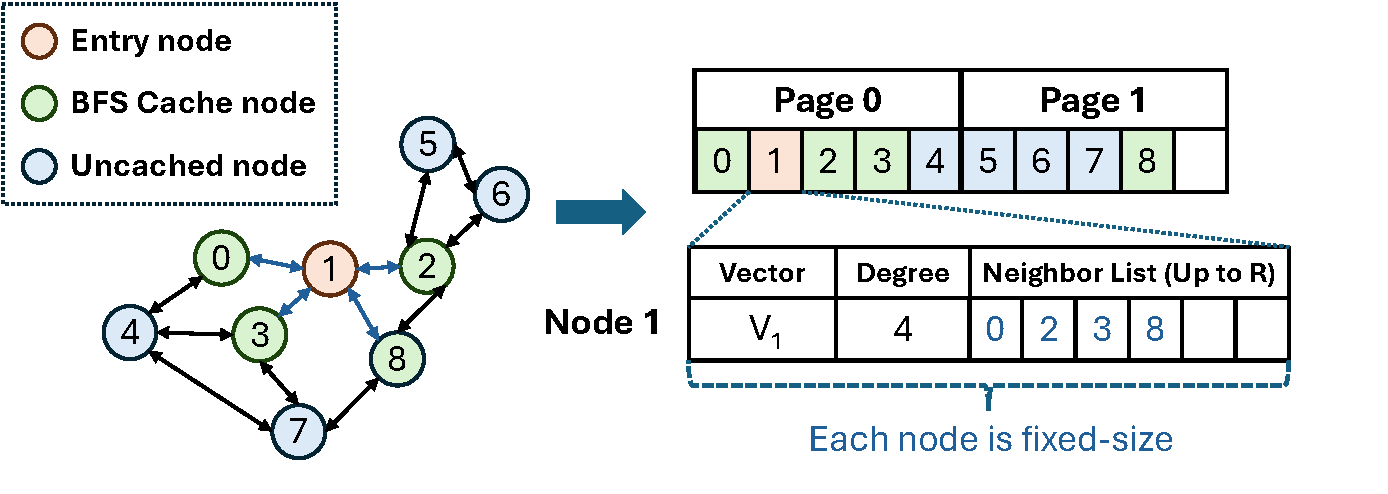
\includegraphics[width=0.9\textwidth]{img/diskann_layout.pdf}
  \caption[DiskANN disk-index layout]{DiskANN's disk-index layout. Each node is a fixed-length record containing the full-precision vector, the neighbor count, and a fixed-length neighbor-ID list padded as needed. Multiple records are packed into fixed-size sectors, and node IDs are implied by position. Each beam-search hop therefore corresponds to a 4\,KB random read, and the full-precision vector needed for re-ranking is stored together with the neighbor list.}
  \label{fig:diskann-layout}
\end{figure}

\section{Page Layout and Search Reordering}

Another line of work improves disk-based ANN by making each page read more useful.
Starling uses block shuffling to place nearby graph nodes in the same page and builds an in-memory navigation graph to shorten search paths\cite{wang2024starling}.
Select Edges Wisely similarly uses graph-layout decisions guided by monotonic search paths to reduce disk I/O\cite{yue2025selectedges}.
These approaches are effective when the index layout is static and the offline reordering remains representative.
Their benefit can weaken when data is updated, memory budgets shrink, or the query distribution changes.
PaceANN is complementary to this direction because it does not require relayout; it adapts during serving and can be applied to an existing DiskANN index.

\section{Early Termination for ANN Search}

Fixed search budgets waste work on easy queries and may still be insufficient for difficult ones.
Prior work has proposed query-adaptive stopping through learned termination prediction\cite{li2020adaptiveet}, declarative recall targets\cite{chatzakis2025darth}, top-$k$ stability criteria\cite{teofili2025patience}, distance-adaptive beam sizing\cite{aljazzazi2025dabs}, and distribution-aware exploration\cite{zhang2025distributionaware}.
Most of these methods are evaluated on in-memory indexes such as HNSW.
PaceANN instead designs early termination for disk-based serving, where the main objective is to prevent unnecessary expansions from becoming additional SSD reads and queueing delay.
